\subsection{Energy Level Splitting}
The energy splitting of $^{87} {\rm Rb}$ ground state and the first excited state can be found in Fig.~(\ref{fig:D1andD2}) from \cite{steck2001rubidium}, it is a great source of $^{87} {\rm Rb}$ D lines data.

For the ground state of $^{87} {\rm Rb}$, the quantum number of orbital angular momentum ${\bf L}$ is 0 and the first excited state $L = 1$. When we consider the spin of the single electron in the outer shell of the atom, $S = 1/2$, and the interaction between spin and orbital angular momentum ${\bf L} \cdot {\bf S}$, the excited state splits into a fine-structure doublet. The eigenvalue of total electron angular momentum 
\begin{equation}
    {\bf J} = {\bf L} + {\bf S}    
\end{equation}
becomes a good quantum number. For the ground state,  $L = 0$, $S = 1/2$, and $J = 1/2$. The ground state is labeled as $5^2S_{1/2}$ where the atomic states are described by term symbols of the form
\begin{equation}
    ^{2S+1}L_J.
\end{equation}
The interaction between the spin and the orbital angular momentum splits the excited state into doublet $5^2P_{1/2}$ and $5^2P_{3/2}$. The transition between the ground state and the excited state is split into two lines, D1 line($5^2S_{1/2} \rightarrow 5^2P_{1/2}$) and D2 line ($5^2S_{1/2} \rightarrow 5^2P_{3/2}$).

Accounting for nuclear angular momentum ${\bf I}$, the states further split into hyperfine states and are represented in the basis of the total angular momentum
\begin{equation}
    {\bf F} = {\bf J} + {\bf I}.    
\end{equation}
The quantum number of the nuclear spin of $^{87} {\rm Rb}$ is 3/2, as shown in Fig.~(\ref{fig:D1andD2}), the $^{87} {\rm Rb}$ ground state $5^2S_{1/2}$ splits into hyperfine states $\ket{F=1}$ and $\ket{F=2}$. The excited state $5^2P_{1/2}$ splits into hyperfine states $\ket{F=1}$ and $\ket{F=2}$. And the excited state $5^2P_{3/2}$ splits into hyperfine states $\ket{F=1}, \ket{F=2},\ket{F=3}$ and $\ket{F=4}$. The Hamiltonian that leads to the hyperfine split consists of magnetic dipole interaction and electric quadrupole interaction,
\begin{equation}
    \hat{H}_{hfs} = A_{hfs}{\bf I}\cdot{\bf J} + B_{hfs}\frac{3({\bf I}\cdot{\bf J})^2 + 3/2{\bf I}\cdot{\bf J} - I(I+1)J(J+1)}{2I(2I-1)2J(2J-1)}.
\end{equation}
Here $A_{hfs}$ is the magnetic dipole constant and $B_{hfs}$ is the electric quadrupole constant. The hyperfine energy splits for the states are
\begin{equation}
    \Delta E_{hfs} = \frac{1}{2}A_{hfs}K + B_{hfs}\frac{3/2K(K+1) - 2I(I+1)J(J+1)}{2I(2I-1)2J(2J-1)}
\end{equation}
where 
\begin{equation}
    K = F(F+1) - I(I+1) - J(J+1).
\end{equation}
The numerical results of hyperfine states energy can be found in Fig.~(\ref{fig:D1andD2}), they are calculated given the experimental measurement of $A_{hfs}$ and $B_{hfs}$ \cite{bize1999high,ye1996hyperfine,barwood1991frequency}.
\begin{figure}[htbp]
    \centering
    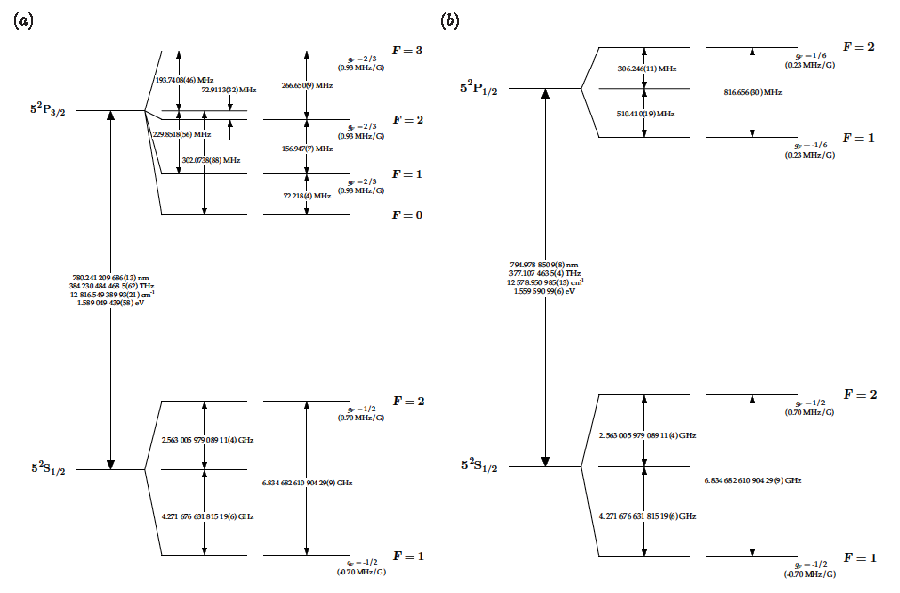
\includegraphics[width=\textwidth]{Chapter2_secs/D1andD2.pdf}
    \caption{Energy splitting of the $^{87} {\rm Rb}$ ground state and the first excited state. }
    \label{fig:D1andD2}
\end{figure}